\definecolor{barblue}{RGB}{38,87,139}
\definecolor{bargrid}{RGB}{205,210,216}

\resizebox{0.88\linewidth}{!}{%
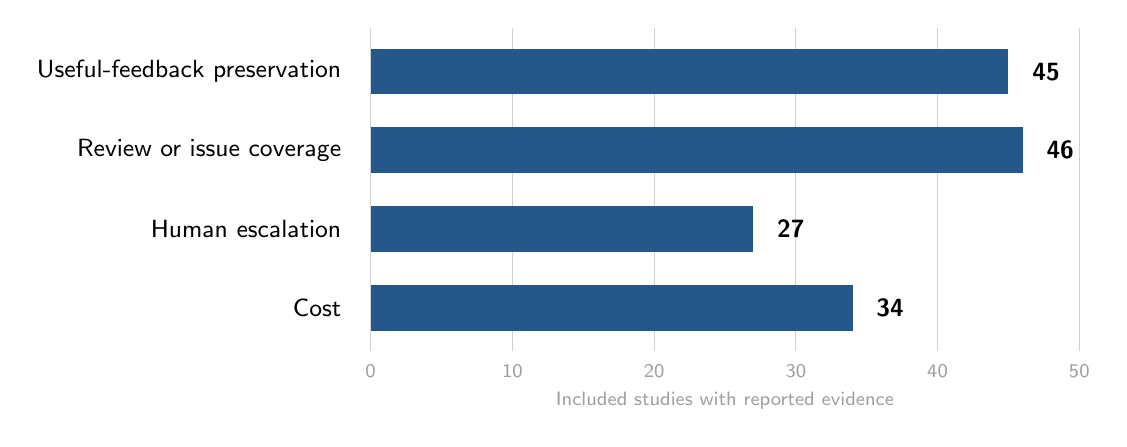
\begin{tikzpicture}[font=\sffamily\small]
  \def\barunit{0.18}
  \def\barheight{0.58}

  \foreach \x in {0,10,20,30,40,50} {
    \draw[bargrid, line width=0.35pt] ({3.6+\x*\barunit},0.25) -- ({3.6+\x*\barunit},4.35);
    \node[font=\sffamily\scriptsize, text=gray!75] at ({3.6+\x*\barunit},0) {\x};
  }

  \node[anchor=east] at (3.35,3.80) {Useful-feedback preservation};
  \node[anchor=east] at (3.35,2.80) {Review or issue coverage};
  \node[anchor=east] at (3.35,1.80) {Human escalation};
  \node[anchor=east] at (3.35,0.80) {Cost};

  \fill[barblue] (3.6,3.51) rectangle ({3.6+45*\barunit},4.09);
  \fill[barblue] (3.6,2.51) rectangle ({3.6+46*\barunit},3.09);
  \fill[barblue] (3.6,1.51) rectangle ({3.6+27*\barunit},2.09);
  \fill[barblue] (3.6,0.51) rectangle ({3.6+34*\barunit},1.09);

  \node[anchor=west, font=\sffamily\bfseries\small] at ({3.78+45*\barunit},3.80) {45};
  \node[anchor=west, font=\sffamily\bfseries\small] at ({3.78+46*\barunit},2.80) {46};
  \node[anchor=west, font=\sffamily\bfseries\small] at ({3.78+27*\barunit},1.80) {27};
  \node[anchor=west, font=\sffamily\bfseries\small] at ({3.78+34*\barunit},0.80) {34};

  \node[font=\sffamily\scriptsize, text=gray!75] at (8.1,-0.38) {Included studies with reported evidence};
\end{tikzpicture}%
}
